\documentclass[tikz,border=10pt]{standalone}
\usepackage[utf8]{inputenc}
\usetikzlibrary{automata,positioning,arrows.meta,calc}

\definecolor{stateoff}{HTML}{D9EAF7}
\definecolor{stateon}{HTML}{D9F2D9}
\definecolor{stateblink}{HTML}{FFE6B3}
\definecolor{resetred}{HTML}{C62828}
\definecolor{blueedge}{HTML}{1565C0}
\definecolor{greenedge}{HTML}{2E7D32}
\definecolor{orangeedge}{HTML}{EF6C00}
\definecolor{textgray}{HTML}{263238}

\begin{document}
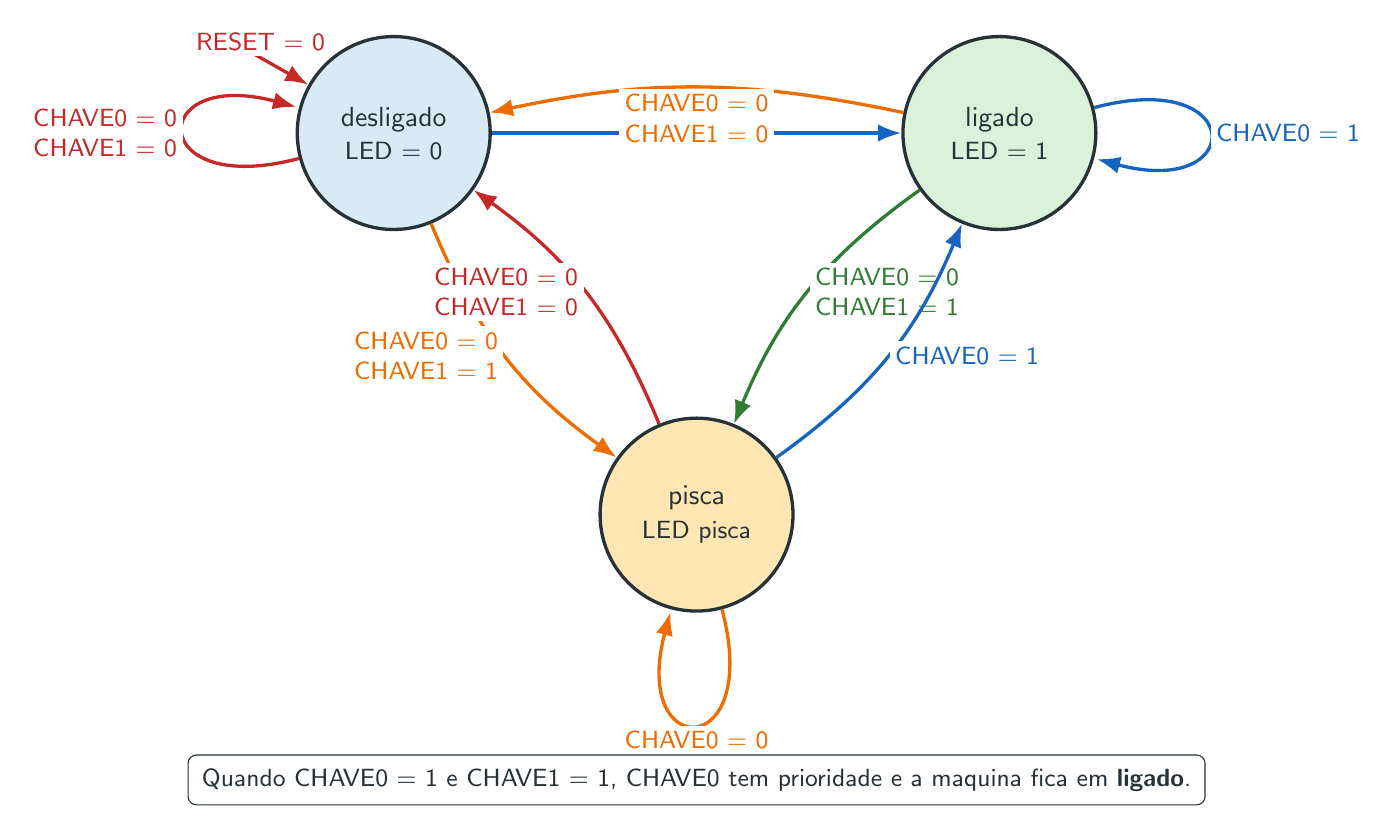
\begin{tikzpicture}[
    >=Latex,
    node distance=5.2cm,
    every node/.style={font=\sffamily},
    state/.style={
        draw=textgray,
        very thick,
        circle,
        minimum size=2.45cm,
        align=center,
        text=textgray
    },
    edge/.style={->, very thick, text=textgray},
    reset/.style={->, very thick, resetred},
    labelbox/.style={
        fill=white,
        inner sep=2pt,
        font=\sffamily\small,
        align=center
    }
]

\node[state, fill=stateoff] (desligado) {desligado\\{\small LED = 0}};
\node[state, fill=stateon, right=of desligado] (ligado) {ligado\\{\small LED = 1}};
\node[state, fill=stateblink, below=3.6cm of $(desligado)!0.5!(ligado)$] (pisca) {pisca\\{\small LED pisca}};

\draw[reset] ($(desligado)+(-2.3,1.3)$) -- node[labelbox, above, text=resetred] {RESET = 0} (desligado);

\draw[edge, blueedge] (desligado) -- node[labelbox, above] {CHAVE0 = 1} (ligado);
\draw[edge, orangeedge] (desligado) to[bend right=16]
    node[labelbox, left] {CHAVE0 = 0\\CHAVE1 = 1} (pisca);
\draw[edge, greenedge] (ligado) to[bend right=16]
    node[labelbox, right] {CHAVE0 = 0\\CHAVE1 = 1} (pisca);

\draw[edge, orangeedge] (ligado) to[bend right=12]
    node[labelbox, below] {CHAVE0 = 0\\CHAVE1 = 0} (desligado);
\draw[edge, blueedge] (pisca) to[bend right=16]
    node[labelbox, right] {CHAVE0 = 1} (ligado);
\draw[edge, resetred] (pisca) to[bend right=16]
    node[labelbox, left] {CHAVE0 = 0\\CHAVE1 = 0} (desligado);

\path[edge, blueedge] (ligado) edge[loop right]
    node[labelbox] {CHAVE0 = 1} (ligado);
\path[edge, orangeedge] (pisca) edge[loop below]
    node[labelbox] {CHAVE0 = 0\\CHAVE1 = 1} (pisca);
\path[edge, resetred] (desligado) edge[loop left]
    node[labelbox] {CHAVE0 = 0\\CHAVE1 = 0} (desligado);

\node[
    font=\sffamily\small,
    align=center,
    text=textgray,
    draw=textgray,
    rounded corners=3pt,
    fill=white,
    inner sep=5pt,
    below=1.8cm of pisca
]
    {Quando CHAVE0 = 1 e CHAVE1 = 1, CHAVE0 tem prioridade e a maquina fica em \textbf{ligado}.};

\end{tikzpicture}
\end{document}
